% Provenance (never printed): the specialisation strand of ../economics_series.md (grade 7). Brief:
% sources/book1/BRIEFS.md, g7-02. Chart data: figdata/grade-7/02-specialisation (WDI SL.AGR.EMPL.ZS,
% NY.GDP.PCAP.PP.KD, SP.POP.TOTL, SL.TLF.TOTL.IN, SL.UEM.TOTL.ZS).
\chapter{Specialisation and the Division of Labour}\label{ch:g7:specialisation}

\begin{openingchart}{Share of all workers employed in farming (with forestry and
fishing) and income per person, in 2024, one dot per country; income on a times-ten
scale.}{World Bank, World Development Indicators, SL.AGR.EMPL.ZS (modelled
estimates of the International Labour Organization) and NY.GDP.PCAP.PP.KD, 2024}
\begin{tikzpicture}
\begin{semilogxaxis}[omincomex, xmin=700, xmax=200000, ymin=0, ymax=100,
  xtickten={-3,...,9}, xlabel={Income per person (dollars of 2021, times-ten scale)},
  ylabel={Percent of workers in farming}]
\addplot table[x=income, y=farm]
  {figdata/grade-7/02-specialisation/out/farm_share_income.csv};
\end{semilogxaxis}
\end{tikzpicture}
\end{openingchart}

% figdata: farm_pairs (BDI 1048 85.4; NER 1796 73.5; ETH 2892 61.0; IND 9416 42.4; CHN 23841 22.2; USA 75698 1.6;
% DEU 62655 1.1; GBR 53412 0.9)
% figdata: facts (countries 171, farm_median_below_5000 47.45, farm_median_above_40000 2.3)
In the poorest countries, most workers are farmers: $85.4\,\%$ of the workers of
Burundi in 2024, $61.0\,\%$ in Ethiopia. In the richest, almost none are: $1.6\,\%$ in
the United States, $0.9\,\%$ in the United Kingdom. Among the countries with an
\omterm{def:g6:living-standards:income-per-person}{income per person} below $5\,000$ dollars, the middle value is about $47\,\%$; above
$40\,000$ dollars, $2.3\,\%$. The dots fall from the upper left to the lower right
almost as one curve.

In a poor village, most families grow their own food and make most of what they use.
In a rich country, a farmer grows one or two crops and buys everything else, and
almost everyone else does one job and buys food from a few farmers. This chapter
explains why doing one thing and exchanging makes people more productive.

\begin{recall}
The three \omterm{def:g6:school-and-work:sector}{sectors of employment} and the move from farms to services were seen in
\cref{ch:g6:school-and-work}; trade between countries in
\cref{ch:g6:a-connected-world}.
\end{recall}

\section{Doing everything yourself}

Imagine a family on a farm far from any town. It grows its grain and vegetables,
keeps a cow and some hens, cuts its wood, builds and mends its house, sews its
clothes and makes its tools. Each member does a little of everything, and does each
task only now and then. Such a family can survive, but it produces little: every
task is done by someone who rarely does it, with simple tools, and much time goes in
moving from one task to the next.

\begin{definition}[Specialisation]\label{def:g7:specialisation:specialisation}
A person, a firm, a region or a country \emph{specialises}\index{specialisation}
when it concentrates on producing a few goods or services, or on a few tasks, and
obtains the rest from others.
\end{definition}

\section{Splitting the task}

\begin{definition}[Division of labour]\label{def:g7:specialisation:division-of-labour}
The \emph{division of labour}\index{division of labour} is the splitting of the
making of one good into separate tasks, each done by a different worker.
\end{definition}

\begin{definition}[Output per worker]\label{def:g7:specialisation:output-per-worker}
\emph{Output per worker}\index{output per worker} is the quantity produced in a
given time divided by the number of workers who produced it:
\[
  \text{output per worker} = \frac{\text{quantity produced}}{\text{number of workers}}.
\]
\end{definition}

\begin{measure}[Output per worker]
For one workshop, \omterm{def:g7:specialisation:output-per-worker}{output per worker} is easy to count: toys made in a day, divided by
the workers. For a whole country, the goods are of thousands of kinds, so they are
added up by their value, as in \cref{ch:g8:gdp}. Output per hour worked is often
better than \omterm{def:g7:specialisation:output-per-worker}{output per worker}, because workers in different countries work different
numbers of hours (\cref{ch:g7:scarcity-and-opportunity-cost}).
\end{measure}

\begin{example}
An invented workshop makes wooden toy trains. Making one train takes four steps:
cutting the pieces (6 minutes), drilling them (4 minutes), assembling (8 minutes)
and painting (6 minutes). A worker who does everything also loses 2 minutes each
time she changes task --- putting away one tool, taking another --- three changes
per train.

\emph{Each worker makes whole trains.} One train takes $6 + 4 + 8 + 6 + 3 \times 2 =
30$ minutes. In a working day of 8 hours, or 480 minutes, a worker makes $480 \div
30 = 16$ trains. Four workers make 64 trains: 16 trains per worker.

\emph{Each worker does one step.} Each now repeats one task all day; with practice,
cutting takes 5 minutes, drilling 4, assembling 6 and painting 5, and no time is lost
changing task. Each worker passes the piece to the next. The line can go no faster
than its slowest station, assembling: one train every 6 minutes, so $480 \div 6 =
80$ trains a day, or $80 \div 4 = 20$ trains per worker. \omterm{def:g7:specialisation:output-per-worker}{Output per worker} rose from
16 to 20 trains, by a quarter, with the same workers, the same tools and the same
hours.
\end{example}

\begin{omfigure}
\begin{tikzpicture}[econ, x=1cm, y=1cm,
  st/.style={draw, rounded corners=2pt, fill=omMeth!12, align=center, font=\scriptsize,
    minimum width=2.1cm, minimum height=1.1cm}]
  \node[st] (a) at (0,0) {cutting\\5 min};
  \node[st] (b) at (3,0) {drilling\\4 min};
  \node[st, fill=omExo!30, very thick] (c) at (6,0) {assembling\\6 min};
  \node[st] (d) at (9,0) {painting\\5 min};
  \draw[-{Stealth}, thick] (a) -- (b);
  \draw[-{Stealth}, thick] (b) -- (c);
  \draw[-{Stealth}, thick] (c) -- (d);
  \draw[-{Stealth}, thick] (d.east) -- ++(0.9,0) node[right, font=\scriptsize] {a train};
  \node[font=\scriptsize, align=center] at (6,-1.15)
    {slowest station: one train\\every 6 minutes, 80 a day};
\end{tikzpicture}

{\small The workshop line of the example, with the time each step takes after
practice. The line can go no faster than its slowest station.}
\end{omfigure}

\section{Why it works: practice, tools, saved time}

The example shows three reasons why the \omterm{def:g7:specialisation:division-of-labour}{division of labour} raises \omterm{def:g7:specialisation:output-per-worker}{output per
worker}.
\begin{itemize}
  \item \textbf{Practice.} A worker who does one task a hundred times a day becomes
        faster and makes fewer mistakes.
  \item \textbf{Saved time.} No time is lost moving from one task, one tool or one
        place to the next.
  \item \textbf{Tools.} When a task is done all day, it pays to build a special tool
        or machine for it, which would be wasted on a task done once a week.
\end{itemize}

\begin{omfigure}
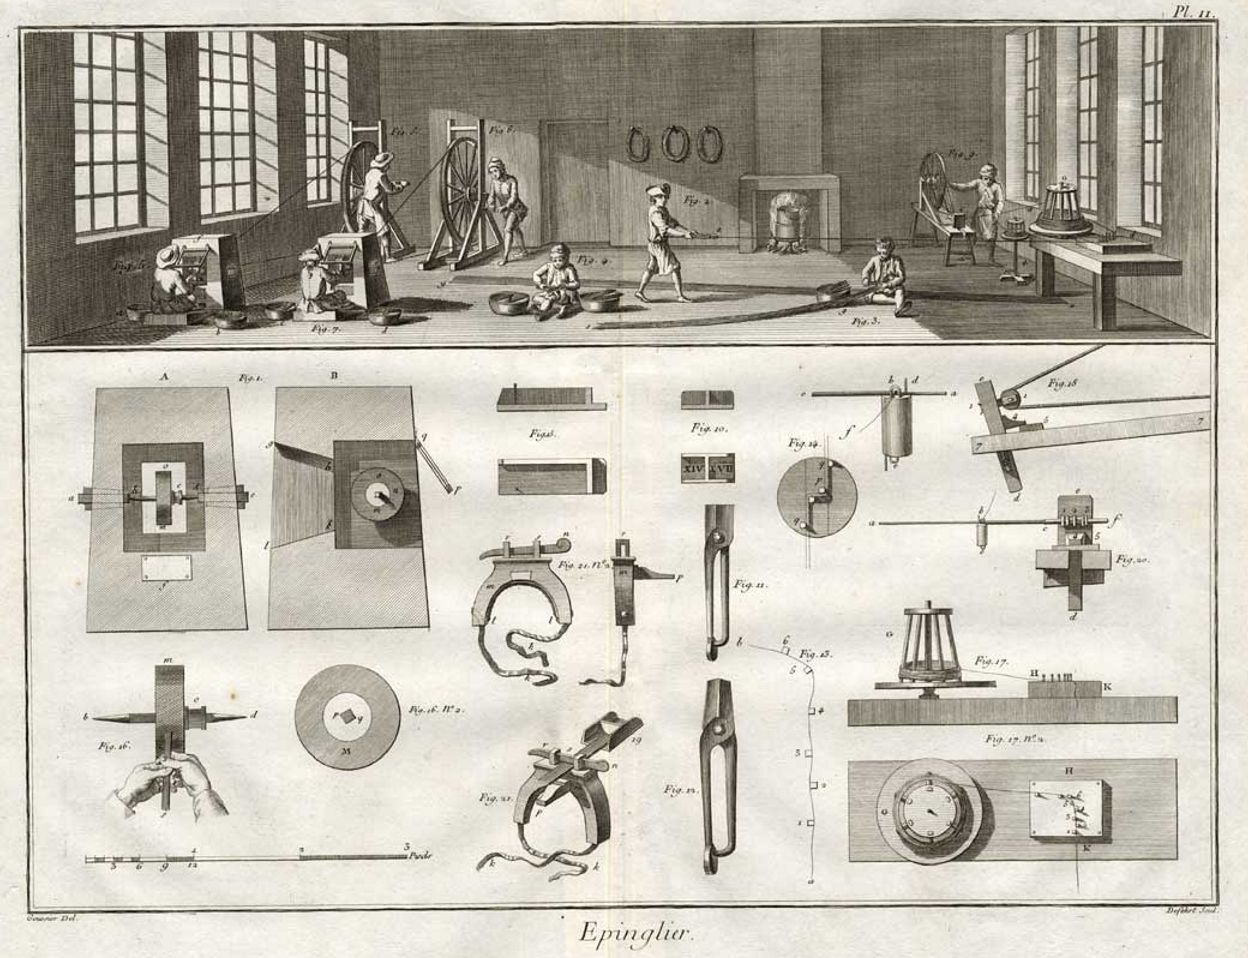
\includegraphics[width=0.72\linewidth]{images/book1/photos/g7-specialisation-pin-making-1762.jpg}

{\small A pin-making workshop in France, engraved in 1762. Each worker does one step:
drawing out the wire on the large wheels, straightening it, cutting it, pointing the
ends on a grinding wheel; the tools of each step are drawn below.}
\end{omfigure}

\section{Specialists need to exchange}

\begin{definition}[Exchange]\label{def:g7:specialisation:exchange}
An \emph{exchange}\index{exchange (voluntary)} is a voluntary transfer in which two
sides each give something to the other: goods for goods, goods for money, or work
for money.
\end{definition}

A worker who paints toy trains all day cannot eat trains. \omterm{def:g7:specialisation:specialisation}{Specialisation} works only
if the specialists can \omterm{def:g7:specialisation:exchange}{exchange} what they make for what they need: the painter is
paid a wage and buys bread, the baker sells bread and buys shoes. Money makes this
easy, because a baker who wants shoes does not have to find a shoemaker who wants
bread.

\begin{omfigure}
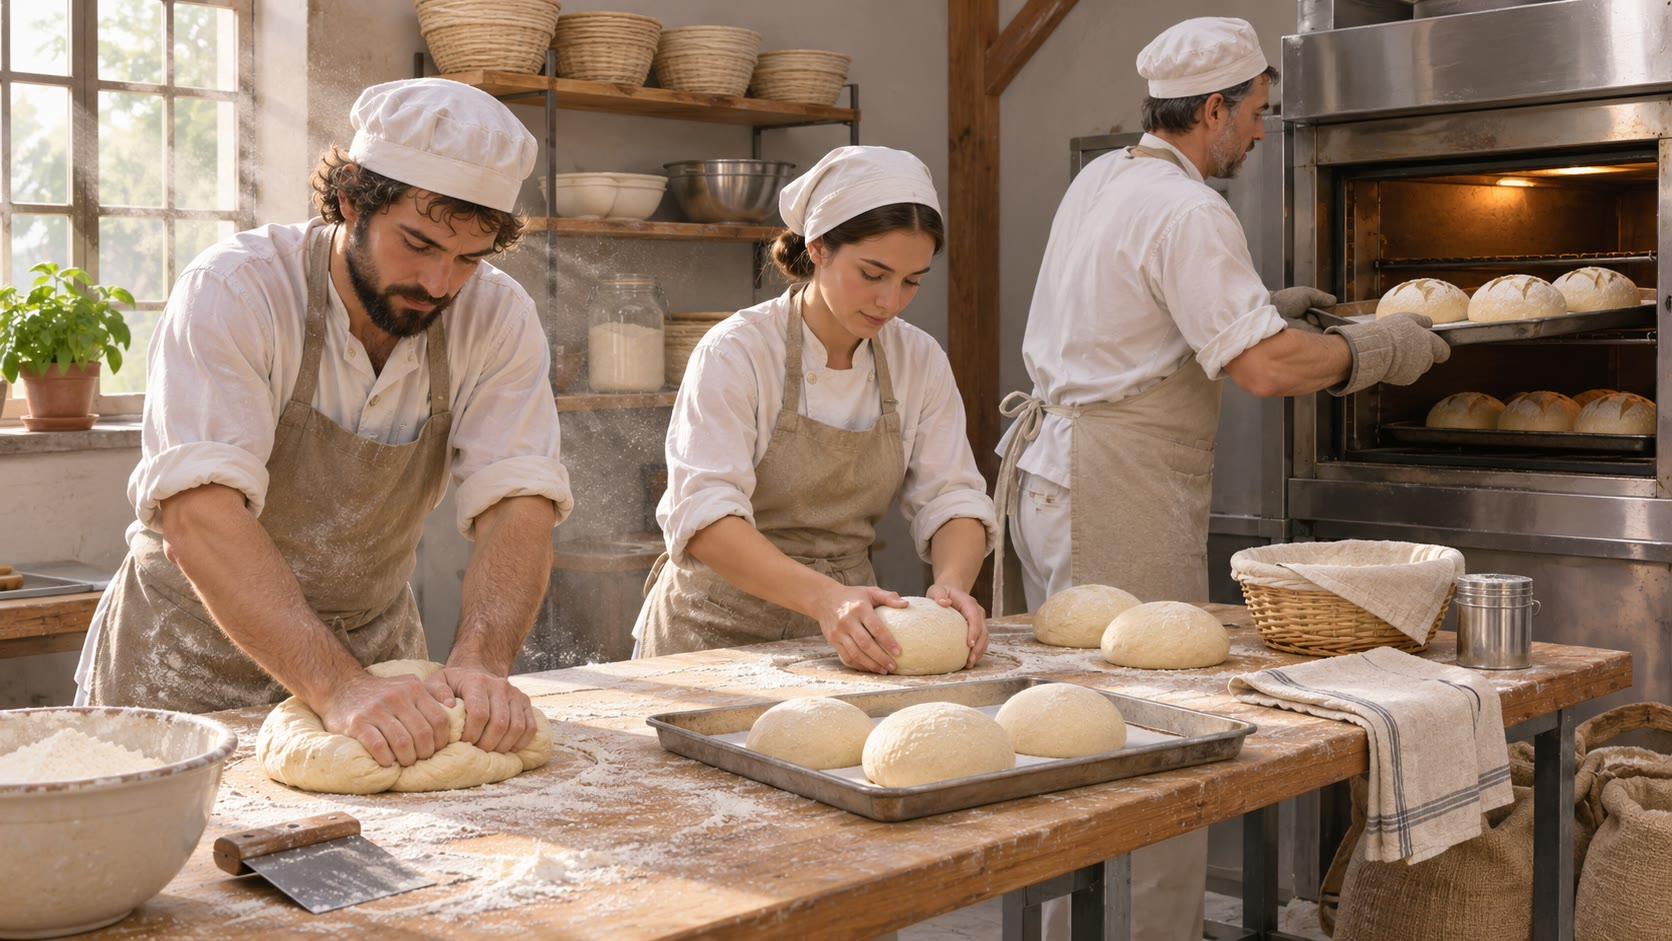
\includegraphics[width=0.55\linewidth]{images/book1/ai/g7-specialisation-bakery-workshop.jpg}

{\small A bakery with three bakers, each at one step: kneading, shaping, baking. The
bread is sold, and the bakers buy everything else.}
\end{omfigure}

% figdata: people_per_farmer (usa 1991 71.8, 2024 129.6; kor 1991 14.7, 2024 34.3; bra 1991 15.9, 2024 27.3;
% chn 1991 3.1, 2024 8.7; ind 1991 4.8, 2024 5.9)
The chart below follows the farmers of five countries: for each farm worker, how
many people live in the country. In the United States, there were $71.8$ people per
farm worker in 1991 and $129.6$ in 2024; in China, $3.1$ and then $8.7$; in India,
$4.8$ and then $5.9$. The number does not say how many people a farmer feeds,
because countries also \omterm{def:g6:a-connected-world:import}{import} and \omterm{def:g6:a-connected-world:export}{export} food. It says how few people are left on
the farms when the others specialise in other work.

\begin{omchart}{People in the population for each worker employed in farming, in five
countries, 1991--2024, on a times-ten scale.}{World Bank, World Development
Indicators: population (SP.POP.TOTL) divided by farm workers, computed as the share of
employment in farming (SL.AGR.EMPL.ZS) times employment, which is the labour force
(SL.TLF.TOTL.IN) minus the unemployed (SL.UEM.TOTL.ZS)}
\begin{tikzpicture}
\begin{semilogyaxis}[omtimesten, xmin=1991, xmax=2024, ymin=1, ymax=300,
  xtick={1991,1995,2000,2005,2010,2015,2020,2024}, xlabel={Year},
  ylabel={People per farm worker},
  legend style={at={(0.5,-0.2)}, anchor=north, legend columns=5}]
\pgfplotsforeachungrouped \col in {usa, kor, bra, chn, ind} {
  \addplot table[x=year, y=\col] {figdata/grade-7/02-specialisation/out/people_per_farmer.csv};
}
\legend{United States, Korea, Brazil, China, India}
\end{semilogyaxis}
\end{tikzpicture}
\end{omchart}

\section{Bigger markets, finer jobs}

A village of 200 people cannot keep a full-time shoemaker busy: it needs a few pairs
of shoes a month. The village cobbler is also a farmer. A town of 20\,000 people
supports several shoemakers, a shop selling only shoes, and perhaps a workshop that
makes only soles. A country of millions supports factories that make only shoe
laces. The larger the market, the finer the \omterm{def:g7:specialisation:division-of-labour}{division of labour} can be.

\begin{model}{Specialisation and the size of the market}
\assumes The making of a good can be split into tasks; workers get faster by
repeating a task; goods can be exchanged at a low cost.
\predicts \omterm{def:g7:specialisation:output-per-worker}{Output per worker} rises as the \omterm{def:g7:specialisation:division-of-labour}{division of labour} gets finer; a larger
market (more buyers within reach) supports more distinct jobs; as \omterm{def:g7:specialisation:output-per-worker}{output per worker}
in farming rises, the share of workers on farms falls.
\tested Across countries, the share of workers in farming falls steadily as income
rises (the opening chart); within countries, the people per farm worker rose in all
five countries of the chart above.
\breaks Tasks that cannot be split (a doctor's diagnosis, a teacher's lesson) or
that depend on the whole being seen by one person; work so repetitive that
attention, and with it quality, falls; markets that are cut off, because transport
is dear, a border is closed or a war breaks out.
\end{model}

\section{Exercises}

\begin{exercise}[$\star$]\label{exo:g7:specialisation:1}
Use the values in the text. What share of workers were in farming in 2024 in Ethiopia,
and in the United States?
\end{exercise}

\begin{exercise}[$\star$]\label{exo:g7:specialisation:2}
One worker makes 12 chairs a week. A team of four workers who split the work makes 60
chairs a week. Compute \omterm{def:g7:specialisation:output-per-worker}{output per worker} in each case.
\end{exercise}

\begin{exercise}[$\star$]\label{exo:g7:specialisation:3}
A tailor makes a shirt in five steps. Each time she changes step she loses 3 minutes.
(a) How many minutes does she lose per shirt? (b) In a week she makes 40 shirts. How
many hours does she lose in all?
\end{exercise}

\begin{exercise}[$\star$]\label{exo:g7:specialisation:4}
Use the values in the text. How many people were there per farm worker in 2024 in the
United States, and in China?
\end{exercise}

\begin{exercise}[$\star\star$]\label{exo:g7:specialisation:5}
A one-person workshop makes stools. Cutting takes 10 minutes, assembling 15 and
varnishing 5, plus 5 minutes lost at each of two changes of task. (a) How many stools
does one worker make in 8 hours? (b) Three workers split the work; with practice the
steps take 8, 12 and 4 minutes, and nobody changes task. How many stools does the line
make in 8 hours? (c) Compute \omterm{def:g7:specialisation:output-per-worker}{output per worker} before and after.
\end{exercise}

\begin{exercise}[$\star\star$]\label{exo:g7:specialisation:6}
In an invented village of 200 people, each person buys one pair of shoes a year. A
full-time shoemaker makes 250 pairs a year. (a) Can the village keep a full-time
shoemaker busy? (b) How many people must a town have to keep four full-time
shoemakers busy?
\end{exercise}

\begin{exercise}[$\star\star$]\label{exo:g7:specialisation:7}
A road opens between a town and a city, and the shoemakers of the town can now sell to
twice as many buyers. According to the model, what happens to the number of different
jobs in the town's shoe trade: more, fewer or the same? Can the model say by how
much?
\end{exercise}

\begin{exercise}[$\star\star$]\label{exo:g7:specialisation:8}
% figdata: facts (farm_chn_1991 59.6, farm_chn_2024 22.2, farm_kor_1991 15.5, farm_kor_2024 5.2)
The share of workers in farming was $59.6\,\%$ in China in 1991 and $22.2\,\%$ in 2024.
In Korea, it was $15.5\,\%$ and $5.2\,\%$. (a) By how many percentage points did it fall
in each country? (b) In which country did it fall by the larger number of times?
\end{exercise}

\begin{exercise}[$\star\star$]\label{exo:g7:specialisation:9}
What observation in a workshop would contradict the model ``\omterm{def:g7:specialisation:specialisation}{Specialisation} and the
size of the market''? Describe it with numbers.
\end{exercise}

\begin{exercise}[$\star\star\star$]\label{exo:g7:specialisation:10}
A line has four stations taking 3, 5, 4 and 3 minutes per piece. (a) How many pieces
does the line make in a 7-hour day? (b) Which station is the bottleneck? (c) A fifth
worker is hired to help at the bottleneck, which now takes $2.5$ minutes. How many
pieces does the line make now, and what is the \omterm{def:g7:specialisation:output-per-worker}{output per worker} before and after?
\end{exercise}

\begin{exercise}[$\star\star\star$]\label{exo:g7:specialisation:11}
A storm cuts the only road between a valley and the rest of the country for a year.
Using the model, predict what happens to the jobs in the valley and to \omterm{def:g7:specialisation:output-per-worker}{output per
worker}. Explain each step.
\end{exercise}

\begin{exercise}[$\star\star\star$]\label{exo:g7:specialisation:12}
Suppose that a country has a low share of workers in farming but also a low \omterm{def:g6:living-standards:income-per-person}{income
per person}. (a) Where would it be on the opening chart? (b) Would that contradict the
model? What else could explain it?
\end{exercise}

\section{Problem: The Bicycle Workshop of Brenmoor}

\begin{problem}[{Weekend problem --- one worker building whole bicycles, four workers
splitting the job, and a doubled market}]
\label{pb:g7:specialisation:1}
Everything in this problem is invented. A workshop in Brenmoor, the capital of
Brenland, builds bicycles. The work has four steps: the frame (70 minutes), the wheels
(50 minutes), the gears and brakes (60 minutes) and the final check (45 minutes). The
working day lasts 8 hours.

\medskip
\noindent\textbf{Part I --- One worker builds whole bicycles.} A worker who builds
whole bicycles also loses 5 minutes at each of the three changes of step.
\begin{enumerate}
  \item How long does one bicycle take this worker?
  \item How many bicycles does one worker build in a 5-day week?
  \item The workshop has four such workers. How many bicycles does it build in a week?
\end{enumerate}

\medskip
\noindent\textbf{Part II --- Four workers split the job.} Each worker now does one step
all day. With practice, the frame takes 48 minutes, the wheels 30, the gears and
brakes 40 and the check 24, and no time is lost changing step.
\begin{enumerate}[resume]
  \item Which step is the bottleneck? How many bicycles does the line build in a day,
        and in a week?
  \item Compute \omterm{def:g7:specialisation:output-per-worker}{output per worker} per week before and after the split, and the \omterm{def:g6:reading-economic-charts:rate-of-change}{rate
        of change} in percent.
  \item The worker at the check is busy only part of the day. How many minutes a day
        is she busy?
  \item Give two reasons why each step became faster.
\end{enumerate}

\medskip
\noindent\textbf{Part III --- Selling to Kestria.} A new trade agreement lets the
workshop sell to Kestria too, and it can sell twice as many bicycles as before. It
splits the work further: eight workers, two on each step, with the frame now taking
40 minutes per worker per bicycle, the wheels 24, the gears and brakes 32 and the
check 20.
\begin{enumerate}[resume]
  \item With two workers on each step, how many minutes does each step need per
        bicycle on the line? (Two workers each taking 40 minutes per frame finish a
        frame every 20 minutes.)
  \item How many bicycles does the line build in a week now?
  \item Compute \omterm{def:g7:specialisation:output-per-worker}{output per worker} per week.
  \item How many workers did the workshop hire, and by what percent did \omterm{def:g7:specialisation:output-per-worker}{output per
        worker} rise compared with Part II?
  \item Can the workshop sell all it builds, if it could sell twice as many as in
        Part II? Explain.
\end{enumerate}
\end{problem}
